\documentclass{article}
\usepackage{amsmath, sfmath, multicol, tkz-euclide, array, enumerate, tcolorbox, tabularray}
\renewcommand{\familydefault}{\sfdefault}
\setlength{\parindent}{0cm}
\pagestyle{empty}
\usepackage[left=1in, top=0.5in, right=1in, bottom=0.5in]{geometry}
\tikzset{>=stealth}
\tcbset{colback=white}

\newcounter{example}[section]
\newenvironment{example}[1][]{\refstepcounter{example}\par\medskip
   {\color{red}\textbf{Example~\theexample. #1}}}{\medskip}

\begin{document}

\section*{Congruent Figures}

\begin{tcolorbox}[colframe=orange!70!white, coltitle=black, title=\textbf{Today I Can}]
\begin{enumerate}
    \item Recognize congruent figures and their corresponding parts.
\end{enumerate}
\end{tcolorbox}

\begin{tcolorbox}[colframe=black!20!white, opacitybacktitle=0.1, coltitle=black, title=\textbf{Congruent Figures}]
Congruent figures have the same shape and same size. \newline

When 2 figures are congruent, you can slide, flip, or turn one so that it fits exactly on the other one.
\end{tcolorbox}

\begin{tcolorbox}[colframe=black!20!white, opacitybacktitle=0.1, coltitle=black, title=\textbf{Congruent Polygons}]
\textbf{Congruent polygons} are polygons with congruent corresponding parts (their matching sides and angles). \newline

\begin{minipage}{0.5\textwidth}
\begin{itemize}
    \item $ABCD \cong EFGH$
    \begin{multicols}{2}
    \begin{itemize}
    \item $\angle A \cong \angle E$ 
    \item $\angle B \cong \angle F$ 
    \item $\angle C \cong \angle G$ 
    \item $\angle D \cong \angle H$
    \end{itemize}
    \begin{itemize}
        \item $\overline{AB} \cong \overline{EF}$
        \item $\overline{BC} \cong \overline{FG}$
        \item $\overline{CD} \cong \overline{GH}$
        \item $\overline{DA} \cong \overline{HE}$
    \end{itemize}
    \end{multicols}
\end{itemize}
\end{minipage}
\begin{minipage}{0.45\textwidth}
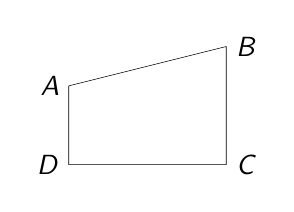
\begin{tikzpicture}
    \tkzDefPoints{0/0/D, 2/0/C, 2/1.5/B, 0/1/A}
    \tkzDrawPolygon(A,B,C,D)
    \tkzLabelPoints[left](A,D)
    \tkzLabelPoints[right](B,C)
    \end{tikzpicture}
    \hspace{0.25in}
    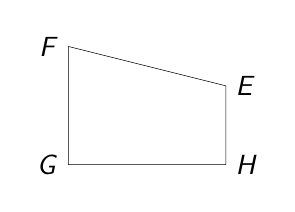
\begin{tikzpicture}
    \tkzDefPoints{0/0/G, 2/0/H, 2/1/E, 0/1.5/F}
    \tkzDrawPolygon(E,F,G,H)
    \tkzLabelPoints[left](F,G)
    \tkzLabelPoints[right](E,H)
\end{tikzpicture}
\end{minipage}
\end{tcolorbox}
\bigskip 

\begin{example}
\begin{enumerate}[(a)]
    \item If $HIJK \cong LMNO$, what are the congruent corresponding parts?    \newline\\    
    \begin{tikzpicture}
    \tkzDefPoints{0/0/H, 1.5/-1/I, 1.75/0.5/J, 0.75/1/K}
    \tkzDrawPolygon(H,I,J,K)
    \tkzLabelPoints[left](H,K)
    \tkzLabelPoints[right](I,J)
    \end{tikzpicture}
    \hspace{0.5in}
    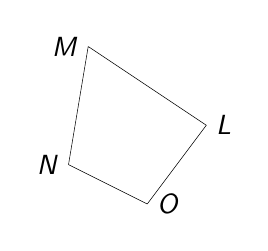
\begin{tikzpicture}[rotate=180]
    \tkzDefPoints{0/0/L, 1.5/-1/M, 1.75/0.5/N, 0.75/1/O}
    \tkzDrawPolygon(L,M,N,O)
    \tkzLabelPoints[right](L,O)
    \tkzLabelPoints[left](M,N)
    \end{tikzpicture}

    \vspace{1in}
    
    \item If $\triangle WYS \cong \triangle MKV$, what are the congruent corresponding parts?
\end{enumerate}
\end{example}
\vspace{1in}

\begin{example}
Suppose $\triangle WYS \cong \triangle MKV$, if $m\angle W=62^\circ$ and $m\angle Y=35^\circ$, what is $m\angle V$? Explain.
\end{example}
\vfill 

\newpage 

In order for 2 polygons to be congruent, \textbf{ALL} pairs of corresponding sides and angles must be congruent.
\newline\\

\begin{example}
\begin{enumerate}[(a)]
    \item Are the triangles congruent? Justify your answer. \newline\\
    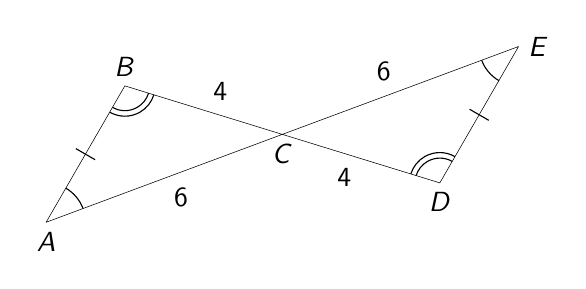
\begin{tikzpicture}
    \tkzDefPoints{0/0/A, 5/0.5/D}
    \tkzDefShiftPoint[A](60:2){B}
    \tkzDefShiftPoint[D](60:2){E}
    \tkzDrawPolygon(A,B,D,E)
    \tkzInterLL(A,E)(D,B)
    \tkzGetPoint{C}
    \tkzLabelSegment[below right](A,C){6}
    \tkzLabelSegment[above left](C,E){6}
    \tkzLabelSegment[above right](B,C){4}
    \tkzLabelSegment[below left](C,D){4}
    \tkzLabelPoints[below](A,C,D)
    \tkzLabelPoints[above](B)
    \tkzLabelPoints[right](E)
    \tkzMarkSegments[mark=|](A,B D,E)
    \tkzMarkAngles[size=0.5](C,A,B C,E,D)
    \tkzMarkAngles[arc=ll, size=0.35](A,B,C E,D,C)
    \end{tikzpicture}
\vspace{1.5in}
    \item Is $\triangle ABD \cong \triangle CBD$? Justify your answer. \newline\\

    \begin{tikzpicture}
    \tkzDefPoints{0/0/A, 1.5/0/B, 3/0/C, 1.5/2/D}
    \tkzDrawPolygon(A,C,D)
    \tkzDrawSegment(D,B)
    \tkzMarkSegments[mark=|](A,D C,D)
    \tkzLabelPoints[below](A,B,C)
    \tkzLabelPoints[above](D)
    \end{tikzpicture}
\end{enumerate}
\end{example}
\vspace{1.5in}

\begin{tcolorbox}[colframe=black!20!white, opacitybacktitle=0.1, coltitle=black, title=\textbf{Third Angle Theorem}]

\begin{minipage}{0.5\textwidth}
    \begin{itemize}
        \item If $\angle A \cong \angle D$ and $\angle B \cong \angle E$, then $\angle C \cong \angle F$.
    \end{itemize}
\end{minipage}
\begin{minipage}{0.45\textwidth}
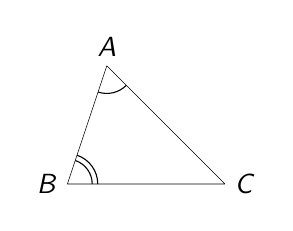
\begin{tikzpicture}
    \tkzDefPoints{0/0/B, 2/0/C, 0.5/1.5/A}
    \tkzDrawPolygon(A,B,C)
    \tkzLabelPoints[left](B)
    \tkzLabelPoints[right](C)
    \tkzLabelPoints[above](A)
    \tkzMarkAngle[size=0.35](B,A,C)
    \tkzMarkAngle[arc=ll, size=0.35](C,B,A)
    \end{tikzpicture}
    \hspace{0.15in}
    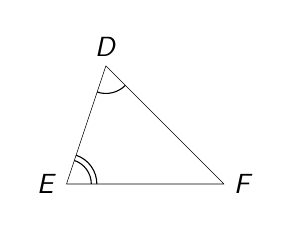
\begin{tikzpicture}
    \tkzDefPoints{0/0/E, 2/0/F, 0.5/1.5/D}
    \tkzDrawPolygon(D,E,F)
    \tkzLabelPoints[left](E)
    \tkzLabelPoints[right](F)
    \tkzLabelPoints[above](D)
    \tkzMarkAngle[size=0.35](E,D,F)
    \tkzMarkAngle[arc=ll, size=0.35](F,E,D)
\end{tikzpicture}
\end{minipage}
\end{tcolorbox}


\end{document}
